% [Overleaf] https://www.overleaf.com/read/bygnpxwcwwjd
% [YouTube] https://youtu.be/dX3F5_RHWRg
% [GitHub] https://github.com/nobucshirai/infona2020_slide_15
\documentclass[dvipdfmx,aspectratio=169,20pt]{beamer}
\usepackage{bxdpx-beamer}

% Beamer theme
\usetheme{Boadilla}

%%%%% JAPANESE FONT SETTINGS %%%%%
\usepackage[utf8]{inputenc}
\usepackage{pxjahyper}
\renewcommand{\kanjifamilydefault}{\gtdefault} % for Gothic Japanese fonts
\newcommand{\myfontsetting}[3]{{\fontsize{#1}{#2}\selectfont #3}}
\usepackage[deluxe,uplatex]{otf} % needed to use super bold Japanese fonts
\usepackage[unicode,noto-otc]{pxchfon} % needed to use super bold Japanese fonts
%%%%%%%%%%%%%%%%%%%%%%%%%%%%%%%%%%

%%%%% SETTINGS FOR MATH SYMBOLS %%%%%
\usepackage{amsmath,amssymb}
\usepackage{bm}
%\usepackage{graphicx}
\usepackage{latexsym}
\usefonttheme{professionalfonts} % use Serif fonts for equations
%%%%%%%%%%%%%%%%%%%%%%%%%%%%%%%%%%%%%

\usepackage{fancybox,ascmac}
\usepackage{url}
\usepackage[many]{tcolorbox}

%%%%% ALGORITHM SETTING %%%%%
\usepackage{algorithm}
\usepackage[noend]{algorithmic}
\algsetup{linenosize=\color{fg!50}\fontsize{8pt}{8pt}\selectfont}
\renewcommand\algorithmicdo{\bfseries :}
\renewcommand\algorithmicthen{\bfseries :}
\renewcommand\algorithmicrequire{\textbf{Input:}}
\renewcommand\algorithmicensure{\textbf{Output:}}
\renewcommand{\algorithmicprint}{\textbf{break}}
%%%%%%%%%%%%%%%%%%%%%%%%%%%%%
\definecolor{myblue1}{RGB}{45,130,200}
\definecolor{myblue2}{RGB}{26,89,142}
\setbeamertemplate{navigation symbols}{}
\setbeamercolor*{structure}{fg=myblue1,bg=blue}
\setbeamercolor{block title}{fg=myblue1!50!black}
\setbeamercolor*{block title example}{fg=white,bg=myblue2}
\setbeamercolor*{palette primary}{use=structure,fg=white,bg=structure.fg}
\setbeamercolor*{palette secondary}{use=structure,fg=white,bg=structure.fg!75!black}
\setbeamercolor*{palette tertiary}{use=structure,fg=white,bg=structure.fg!50!black}
\setbeamercolor*{palette quaternary}{fg=black,bg=myblue1}

\setbeamerfont{alerted text}{series=\bfseries}
\setbeamerfont{section in toc}{series=\mdseries}
\setbeamerfont{frametitle}{size=\Large,series=\bfseries}
\setbeamerfont{title}{size=\LARGE,series=\bfseries}
\setbeamerfont{date}{size=\small}

\setbeamertemplate{block title}[shadow=false]
\setbeamertemplate{blocks}[rounded][shadow=false]

%%%%% BEAMER FOOTLINE SETTINGS %%%%%%
\setbeamertemplate{footline}[frame number]{}
\setbeamerfont{footline}{size=\bf\footnotesize\small}
%%%%%%%%%%%%%%%%%%%%%%%%%%%%%%%%%%%%%

%%%%% BEAMER ITEM SETTINGS %%%%%
\setbeamertemplate{itemize item}[circle]
\setbeamertemplate{itemize subitem}[triangle]
\setbeamertemplate{enumerate item}[circle]
%%%%%%%%%%%%%%%%%%%%%%%%%%%%%%%%

\begin{document}

\graphicspath{{figs/}}

%%%%%%%%%%%%%%%%%%%%%%%%%%%%%%%%
%タイトルページ

\title{\myfontsetting{32pt}{32pt}{偏微分方程式の数値解法 (2)}}

\titlegraphic{\vspace{-7mm}\flushright
\includegraphics[width=1.8cm,height=1.8cm]{hattari_kun_good_org.eps}}

\setbeamertemplate{title page}{%
    \begin{flushright}
        \usebeamercolor[fg]{titlegraphic}\inserttitlegraphic
    \end{flushright}
    \vspace{-0.6cm}
    \hspace{1.5cm}{\selectfont\usebeamerfont{subtitle} \usebeamercolor[fg]{subtitle} [\href{https://youtu.be/dX3F5_RHWRg}{数値解析 第15回}] \par}
    \vspace{0.5cm}
    %\vspace{2.5em}
    {\centering\usebeamerfont{title} \usebeamercolor[fg]{title} \inserttitle \par}
    \vspace{0.5cm}
    \begin{center}
        初期値と境界条件で決まる場の時間発展
    \end{center}
}

\date[\todey]{}

\frame{\titlepage}

%%%%%%%%%%%%%%%%%%%%%%%%%%%%%%%%
\begin{frame}
%%%%% START_TAG B %%%%%
%\noindent{\bf X\hspace{-.1em}I\hspace{-.1em}V-B.}
\frametitle{[問題] X\hspace{-.1em}I\hspace{-.1em}V-B}

\myfontsetting{14pt}{14pt}{
X\hspace{-.1em}I\hspace{-.1em}V-Aで求めた 温度分布 $T(x,y)$ を初期条件 $T(x,y,t=0)$ として鉄板が断熱された環境に移された場合を考える。
時間の経過とともに熱が伝わって一様な温度分布に近づいていく様子を数値的に求める。
解くべき方程式は2次元の熱伝導方程式 $\frac{\partial T(x,y,t)}{\partial t} = a \left\{ \frac{\partial^2 T(x,y,t)}{\partial x^2} + \frac{\partial^2 T(x,y,t)}{\partial y^2}\right\}$ $(0\le x \le 1, 0\le y \le 1)$ である。ここで $a$ は温度伝導率であり $a=1$ とする。
}
\end{frame}

\begin{frame}
\frametitle{[問題] X\hspace{-.1em}I\hspace{-.1em}V-B (続き)}

\myfontsetting{14pt}{14pt}{
両辺をX\hspace{-.1em}I\hspace{-.1em}V-Aと同じ格子点を用いて離散化し、オイラー法を用い時間幅を $\varDelta t=0.001$ として $t=0.001, 0.01, 0.1,1$ での温度分布を求めるプログラムを作成せよ。
温度分布はX\hspace{-.1em}I\hspace{-.1em}V-Aと同様に数値で出力するか等高線を用いた図を作成して示すこと。
}

\myfontsetting{10pt}{10pt}{
作成したプログラムも提出すること。プログラミング言語は問わない。
}

%%%%% END_TAG B %%%%%
\end{frame}
%%%%%%%%%%%%%%%%%%%%%%%%%%%%%%%%
\begin{frame}
\frametitle{[略解] X\hspace{-.1em}I\hspace{-.1em}V-B}

\vspace{-2mm}
\begin{figure}[h]
	\begin{center}
    	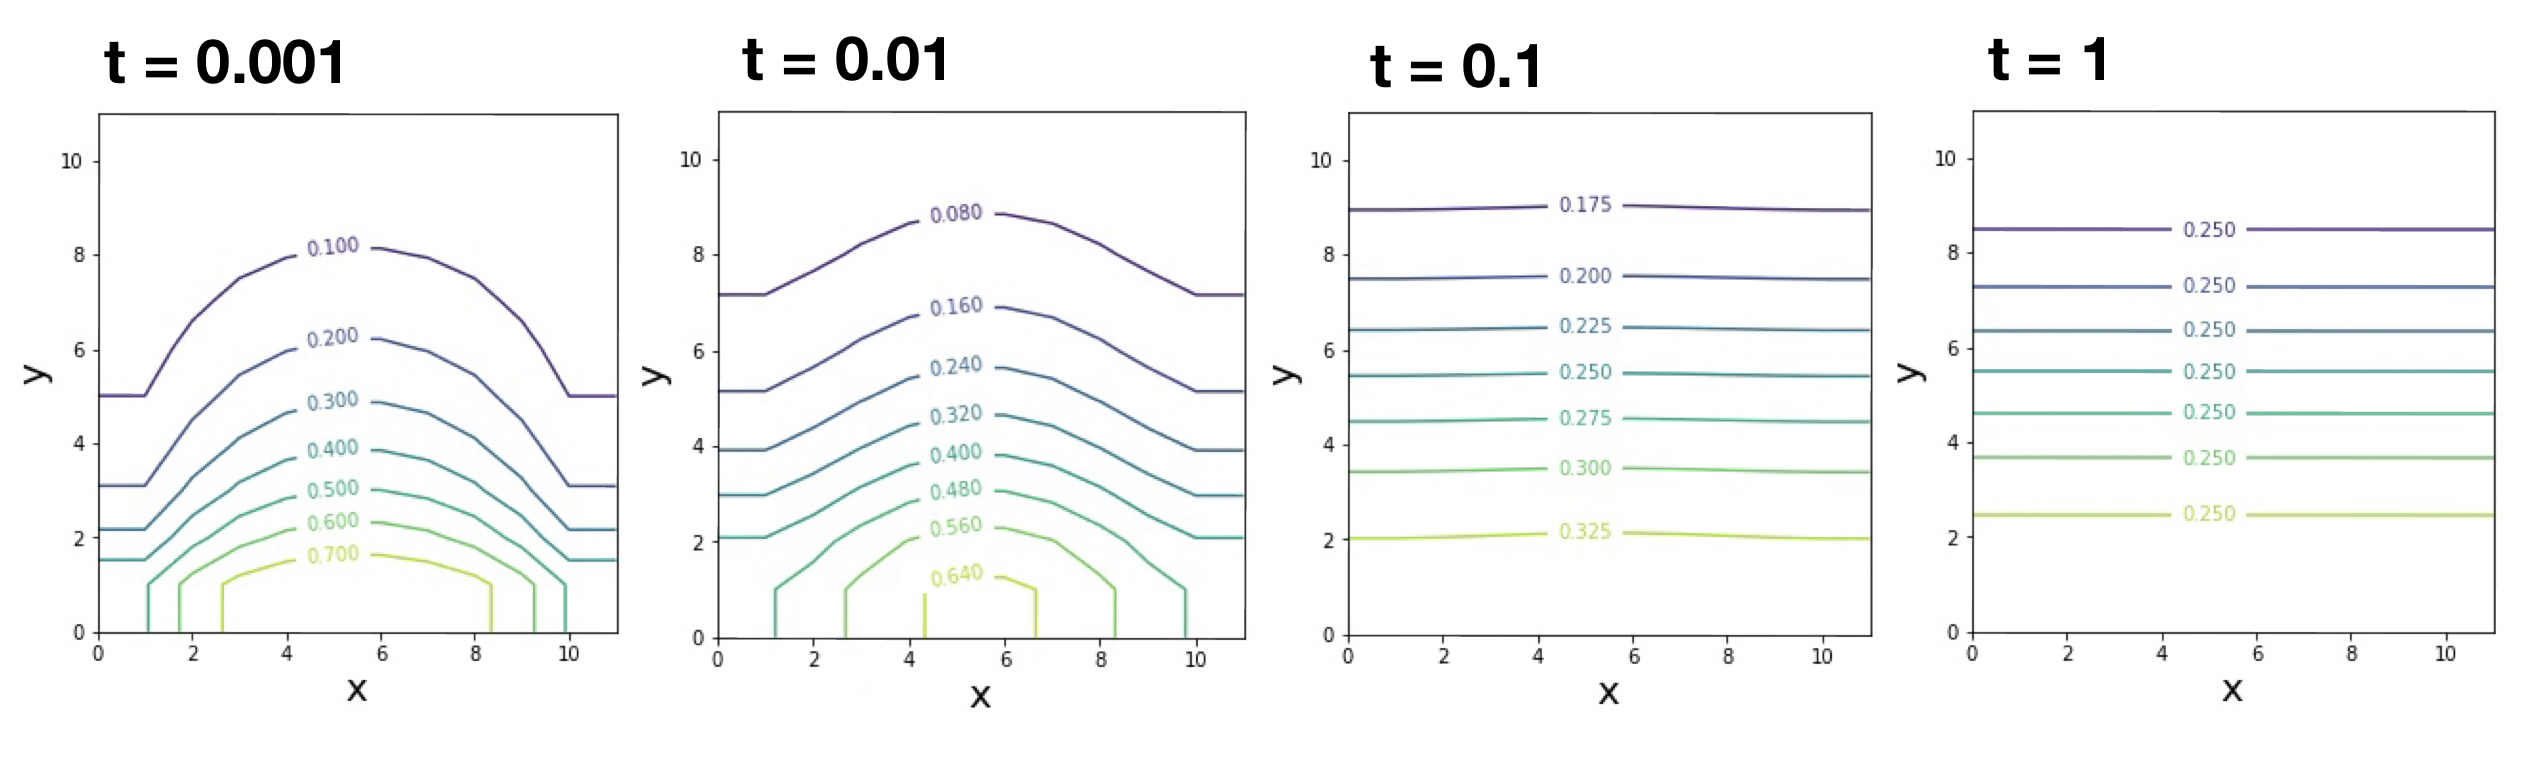
\includegraphics[width=1.0\textwidth]{fig15-1_report15_ans.jpeg}
	\end{center}
\end{figure}

\end{frame}
%%%%%%%%%%%%%%%%%%%%%%%%%%%%%%%%
\begin{frame}
\frametitle{\myfontsetting{24pt}{24pt}{線形偏微分方程式の初期条件と境界条件}}

\begin{itemize}
    \setlength{\itemsep}{0.15cm}
    \item \myfontsetting{16pt}{16pt}{$u(x,t)$ \myfontsetting{12pt}{12pt}{$(0\le x \le L,\, t\ge 0)$} の場合}
    \item \myfontsetting{16pt}{16pt}{初期条件}
    \begin{itemize}
\vspace{1mm}
        \item \myfontsetting{14pt}{14pt}{$u(x,0) = f(x)$} \hspace{3mm} \myfontsetting{10pt}{10pt}{[$f(x)$ を{\bf コーシー (Cauchy) データ}とよぶ]}
    \end{itemize}
    \item \myfontsetting{16pt}{16pt}{第1種境界条件} \myfontsetting{10pt}{10pt}{\bf [ディリクレ (Dirichlet) 条件]}
    \begin{itemize}
\vspace{1mm}
        \item \myfontsetting{14pt}{14pt}{$u(0,t) = c_0,\, u(L,t) = c_L$}
    \end{itemize}
    \item \myfontsetting{16pt}{16pt}{第2種境界条件} \myfontsetting{10pt}{10pt}{\bf [ノイマン (Neumann) 条件]}
\vspace{1mm}
    \begin{itemize}
        \item \myfontsetting{14pt}{14pt}{$\displaystyle \left.\frac{\partial u(x,t)}{\partial x}\right|_{x=0} = C_0,\quad \left.\frac{\partial u(x,t)}{\partial x}\right|_{x=L} = C_L$}
    \end{itemize}
\end{itemize}
\end{frame}
%%%%%%%%%%%%%%%%%%%%%%%%%%%%%%%%
\begin{frame}{{\myfontsetting{22pt}{22pt}{[手法] 偏微分方程式の初期値問題の解法}}}
\begin{block}{\myfontsetting{16pt}{16pt}{\bf\small オイラー法を用いた熱伝導方程式の数値解法}}
    \myfontsetting{15pt}{18pt}{
    \begin{algorithmic}[1]
        \label{alg:heat_equation}
        \REQUIRE $k_\mathrm{max}$, $N$, $h = \frac{1}{N+1}$, $\varDelta t$, $T_{ij}$ \myfontsetting{8pt}{8pt}{$(0\le i, j \le N+1)$} \myfontsetting{8pt}{8pt}{[初期値]}
        \ENSURE $T_{ij}$
		\FOR{$k = 1,2, \dots, k_\mathrm{max}$}
        \STATE \myfontsetting{12pt}{12pt}{$\mathrm{T\_BULK\_UPDATE}(N,T,T^{\textrm{+}})$} \hspace{2mm} \myfontsetting{8pt}{8pt}{(p.~\ref{func:T_BULK_UPDATE})} \label{op:T_BULK_UPDATE}
        \STATE \myfontsetting{12pt}{12pt}{$\mathrm{T\_BOUNDARY\_UPDATE}(N,T)$} \hspace{2mm} \myfontsetting{8pt}{8pt}{(p.~\ref{func:T_BOUNDARY_UPDATE})} \label{op:T_BOUNDARY_UPDATE}
        \STATE \myfontsetting{12pt}{12pt}{$\mathrm{T\_CORNER\_POINTS\_UPDATE}(N,T)$} \hspace{2mm} \myfontsetting{8pt}{8pt}{(p.~\ref{func:T_CORNER_POINTS_UPDATE})} \label{op:T_CORNER_POINTS_UPDATE}
        \ENDFOR
    \end{algorithmic}
    }
\end{block}
\end{frame}
%%%%%%%%%%%%%%%%%%%%%%%%%%%%%%%%
\begin{frame}{{\myfontsetting{22pt}{22pt}{[手法] バルク部分の温度更新}
\myfontsetting{18pt}{18pt}{(p.~\ref{alg:heat_equation}, $\mathbf{\ell}$.~\ref{func:T_BULK_UPDATE})}
\\
\vspace{-7mm}
\myfontsetting{8pt}{8pt}{※ 「バルク (BULK)」は対象物の境界から十分内側を指す用語だがここでは境界以外をバルクと呼ぶ。}
}}

\begin{block}{\myfontsetting{10pt}{12pt}{$\mathrm{T\_BULK\_UPDATE}(N,T,T^{\textrm{+}})$} \label{func:T_BULK_UPDATE}}
    \myfontsetting{10pt}{12pt}{
    \begin{algorithmic}[1]
        \FOR{$i = 1,\dots, N$}
        \FOR{$j = 1,\dots, N$}
		\STATE $S \leftarrow 0$; $c \leftarrow 0$
		\IF{$i \ge 2$}
		\STATE $S \leftarrow S + T_{i-1,j}$; $c \leftarrow c + 1$
		\ENDIF
		\IF{$i \le N-1$}
		\STATE $S \leftarrow S + T_{i+1,j}$; $c \leftarrow c + 1$
		\ENDIF
		\IF{$j \ge 2$}
		\STATE $S \leftarrow S + T_{i,j-1}$; $c \leftarrow c + 1$
		\ENDIF
		\IF{$j \le N-1$}
		\STATE $S \leftarrow S + T_{i,j+1}$; $c \leftarrow c + 1$
		\ENDIF
		\STATE $T^{\textrm{+}}_{ij} \leftarrow \left\{ 1 - \frac{c\, \varDelta t}{h^2} \right\} T_{ij} + \frac{\varDelta t}{h^2}S$
        \ENDFOR
        \ENDFOR
        \FOR{$i = 1,\dots, N$}
        \FOR{$j = 1,\dots, N$}
		\STATE $T_{ij} \leftarrow T^{\textrm{+}}_{ij}$
        \ENDFOR
        \ENDFOR
    \end{algorithmic}
    }
\end{block}
\end{frame}

%\vspace{-7mm}
%
%\myfontsetting{8pt}{8pt}{※ 「バルク部分」とは本来対象物(本問では鉄板)境界から十分内側の部分を指す用語だが、ここでは境界部分以外の部分をバルク (BULK) と呼んでいる。}

%%%%%%%%%%%%%%%%%%%%%%%%%%%%%%%%
\begin{frame}{{\myfontsetting{22pt}{22pt}{[手法] 境界部分の温度更新}
\myfontsetting{18pt}{18pt}{(p.~\ref{alg:heat_equation}, $\mathbf{\ell}$.~\ref{func:T_BOUNDARY_UPDATE})}
}}

\begin{block}{\myfontsetting{15pt}{15pt}{$\mathrm{T\_BOUNDARY\_UPDATE}(N,T)$} \label{func:T_BOUNDARY_UPDATE}}
    \myfontsetting{14pt}{16pt}{
    \begin{algorithmic}[1]
        \FOR{$i = 1,\dots, N$}
		\STATE $T_{i0} \leftarrow T_{i1}$
		\STATE $T_{i,N+1} \leftarrow T_{iN}$
        \ENDFOR
        \FOR{$j = 1,\dots, N$}
		\STATE $T_{0j} \leftarrow T_{1j}$
		\STATE $T_{N+1,j} \leftarrow T_{Nj}$
        \ENDFOR
    \end{algorithmic}
    }
\end{block}
\end{frame}
%%%%%%%%%%%%%%%%%%%%%%%%%%%%%%%%
\begin{frame}{{\myfontsetting{22pt}{22pt}{[手法] 四隅の点の温度更新}
\myfontsetting{18pt}{18pt}{(p.~\ref{alg:heat_equation}, $\mathbf{\ell}$.~\ref{func:T_CORNER_POINTS_UPDATE})}
}}

\begin{block}{\myfontsetting{15pt}{15pt}{$\mathrm{T\_CORNER\_POINTS\_UPDATE}(N,T)$} \label{func:T_CORNER_POINTS_UPDATE}}
    \myfontsetting{14pt}{16pt}{
    \begin{algorithmic}[1]
		\STATE $T_{00} \leftarrow \frac{1}{2}\left(T_{01}+T_{10}\right)$
		\STATE $T_{0,N+1} \leftarrow \frac{1}{2}\left(T_{0N}+T_{1,N+1}\right)$
		\STATE $T_{N+1,0} \leftarrow \frac{1}{2}\left(T_{N+1, 1}+T_{N,0}\right)$
		\STATE $T_{N+1,N+1} \leftarrow \frac{1}{2}\left(T_{N+1, N}+T_{N,N+1}\right)$
    \end{algorithmic}
    }
\end{block}
\end{frame}
%%%%%%%%%%%%%%%%%%%%%%%%%%%%%%%%
\begin{frame}

\vspace{10mm}

\begin{center}
    \myfontsetting{36pt}{36pt}{\bf \color{myblue1} 修正前のコード}
    
    \vspace{5mm}
    
    \begin{flushleft}
    \myfontsetting{12pt}{12pt}{ ※ 2021/1/21 に配信した授業で説明した「(境界条件を考慮していない)偏微分方程式の初期値問題の解法」を次ページに残しておく。}
    
    \vspace{2.5mm}
    
    \myfontsetting{12pt}{12pt}{ ※ 以下のアルゴリズムでは境界における $T(x,y)$ の値を常に0と設定しているため断熱の条件ではなく $T=0$ の熱源と接している状態になっているため時間を進めても鉄板全体の温度が一定にならず中心部に残った熱がだんだん消えていく時間発展となる。}
    \end{flushleft}
\end{center}
\end{frame}
%%%%%%%%%%%%%%%%%%%%%%%%%%%%%%%%
\begin{frame}{{\myfontsetting{22pt}{22pt}{[手法] 偏微分方程式の初期値問題の解法}}}
\begin{block}{\myfontsetting{15pt}{15pt}{\bf\small オイラー法を用いた熱伝導方程式の数値解法}}
    \myfontsetting{8pt}{10pt}{
    \begin{algorithmic}[1]
        \REQUIRE $k_\mathrm{max}$, $N$, $h = \frac{1}{N+1}$, $\varDelta t$, $T_{ij}$ \myfontsetting{8pt}{8pt}{$(0\le i, j \le N+1)$} \myfontsetting{8pt}{8pt}{[初期値]}
        \ENSURE $T_{ij}$
		\FOR{$k = 1,2, \dots, k_\mathrm{max}$}
        \FOR{$i = 0,\dots, N+1$}
        \FOR{$j = 0,\dots, N+1$}
		\STATE $S \leftarrow 0$
		\IF{$i-1\ge 0$}
		\STATE $S \leftarrow S + T_{i-1,j}$
		\ENDIF
		\IF{$i+1 \le N+1$}
		\STATE $S \leftarrow S + T_{i+1,j}$
		\ENDIF
		\IF{$j-1\ge 0$}
		\STATE $S \leftarrow S + T_{i,j-1}$
		\ENDIF
		\IF{$i+1 \le N+1$}
		\STATE $S \leftarrow S + T_{i,j+1}$
		\ENDIF
		\STATE $U_{ij} \leftarrow \left\{ 1 - \frac{4\varDelta t}{h^2} \right\} T_{ij} + \frac{\varDelta t}{h^2}S$
        \ENDFOR
        \ENDFOR
        \FOR{$i = 0,\dots, N+1$}
        \FOR{$j = 0,\dots, N+1$}
		\STATE $T_{ij} \leftarrow U_{ij}$
        \ENDFOR
        \ENDFOR
        \ENDFOR
    \end{algorithmic}
    }
\end{block}
\end{frame}
%%%%%%%%%%%%%%%%%%%%%%%%%%%%%%%%

\end{document}
